\section{Support Vector Machines (SVM)}
\begin{figure}[H]
	\captionsetup{width=15cm,font=small}
	\begin{center}
		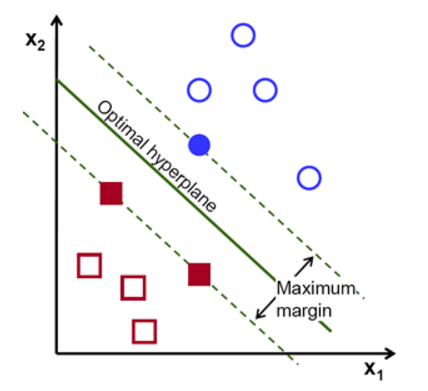
\includegraphics[width=15cm,height=10cm]{optimal_margin_svm}
		\caption[Support Vector Machine optimal hyperplane]{Visual representation taken from \cite{itseez2014theopencv} for the optimal hyperplane and the maximum margin that characterizes the SVM}
		\label{fig:optimal_margin_svm}
	\end{center}
\end{figure}
A Support Vector Machine (SVM) is a discriminative classifier formally defined by a separating hyperplane. Based on training data, the algorithm outputs an optimal hyperplane which categorizes new examples. Formally, a hyperplane is defined as:
\begin{align}
	|\beta_{0} + \beta^{T}x| = 1
\end{align}
where $\beta$ is known as the weight vector and $\beta_{0}$ as the bias.
By convention, the optimal hyperplane is represented as
\begin{align}
	|\beta_{0} + \beta^{T}x| = 1
\end{align}
where $x$  symbolizes the training examples closest to the hyperplane. These training examples are called \textbf{support vectors}. 

The problem that the SVM tries to solve is to find the values for $\beta$ and $\beta_{0}$ so that the distance between the support vectors and the hyperplane is maximum. Generally, the distance between a point $x$ and a hyperplane $(\beta, \beta_{0})$ is:
\begin{align}
d = \frac{|\beta_{0} + \beta^{T}x|}{||\beta||}
\end{align}
For the support vectors, this distance becomes
\begin{align}
d_{support\ vectors} = \frac{1}{||\beta||}
\end{align}
Therefore, the margin that can be seen in figure \ref{fig:optimal_margin_svm} is twice the distance to the closes examples:
\begin{align}
M = \frac{2}{||\beta||}
\end{align}
As stated above, the SVM problem consists of maximizing $M$ which is equivalent to the following optimization problem of minimizing the function $L(\beta)$:
\begin{align}
min_{\beta, \beta_{0}} = \frac{1}{2}||\beta||^2\ subject\ to\ y_i(\beta^T x_{i} + \beta_{0}) \geq 1\ ,\forall i
\end{align}
where the constraints model the requirement for the hyperplane to classify correctly all training examples $x_i$ with $y_i$ representing each of the labels of the training examples.
\section{Convolutional Neural Networks (CNN)}